% +--------------------------------------------------------------------+
% | Sample Chapter 2
% +--------------------------------------------------------------------+

\cleardoublepage

% +--------------------------------------------------------------------+
% | Replace "This is Chapter 2" below with the title of your chapter.
% | LaTeX will automatically number the chapters.
% +--------------------------------------------------------------------+

\chapter{OpenGL y Direct3D}
\label{makereference2}

El objetivo de este capítulo es explicar en qué consiste OpenGl, así como su
pipeline de gráficos, los tipos de shaders que incluye y las diferencias que
presenta con DirectX, su principal competidor.

\section{¿Qué es?}
\label{makereference2.1}

OpenGL~\cite{OpenGL} se define como una API \textit{(application programming interface)}, que
es simplemente una librería de software para acceder a capacidades del hardware
de gráficos (ver \citet{Shreiner:2009:OPG:1696492}).

OpenGL está diseñado como una interfaz independiente del hardware que puede ser
implementada en muchos sistemas hardware de gráficos diferentes, o completamente
como software, en el caso de que el sistema no posea hardware de gráficos.
OpenGL no proporciona ninguna funcionalidad para describir modelos en tres
dimensiones ni operaciones para leer ficheros (como imágenes JPEG, por ejemplo).
En su lugar, se deben construir los objetos tridimensionales a partir de un
pequeño conjunto de primitivas geométricas---puntos, líneas, triángulos y
parches.---

\section{Breve historia de OpenGL}
\label{makereference2.2}

OpenGL nace a principios de los años 90, desarrollada por Silicon Graphics~(SGI).  En
los años 80, Silicon Graphics poseía una API privada denominada IRIS GL,
utilizada para producir gráficos en sus estaciones de trabajo IRIS.
Posteriormente, debido a la pérdida de cuota de mercado, decidió hacer su API
pública. Sin embargo, a causa de problemas con patentes y el hecho de tener
características poco relevantes para los gráficos 3D como la funcionalidad de
ventanas, se decidió reescribir algunas de las partes y se lanzó lo que ahora se
conoce como OpenGL.

Esta nueva especificación consiguió logros importantes para la informática gráfica,
como estandarizar el acceso al hardware gráfico, trasladar a los fabricantes la
responsabilidad del desarrollo de las interfaces con el hardware y delegar la
funcionalidad de ventanas al sistema operativo. Todo esto supuso un gran impacto
en la industria, al ofrecer a los desarrolladores una plataforma de alto nivel
sobre la que trabajar.

En 1992, Silicon Graphics lideró la creación del OpenGL Architecture Review
Board (OpenGL ARB)~\cite{OpenGLARB}, un grupo de empresas del sector que sería la encargada de
mantener y extender la especificación en los años siguientes. El OpenGL ARB
estaba formado por 3Dlabs, Apple, ATI, Dell, IBM, Intel, Nvidia, SGI and Sun
Microsystems.

En otoño de 2006, el OpenGL ARB y los directores de Khronos votaron para transferir el
control de OpenGL a Khronos Group. El secretario de la ARB Jon Leech observó:
\textit{``Hemos decidido mover OpenGL a Khronos para asegurar la salud futura de
OpenGL en todas sus formas.''}~\cite{OpenGLARB}

\section{Diseño de OpenGL}
\label{makereference2.3}

OpenGL implementa el llamado pipeline de gráficos o pipeline de renderizado.
Este pipeline consiste en una secuencia de etapas de procesamiento para
convertir datos de una aplicación en una imagen final renderizada. 

\begin{figure}[h]
		\centering
		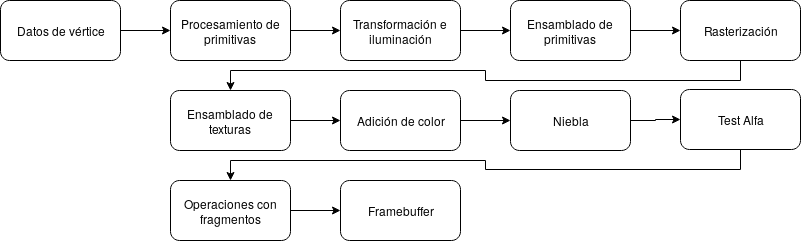
\includegraphics[height=7cm,width=\textwidth]{figures/pipelinefijo.png}
		\caption{Pipeline no programable. OpenGL 1.5}
		\label{fig2.1}
\end{figure}

En un principio, este pipeline de renderizado consistía en varias etapas fijas y
no programables, en las que el programador simplemente elegía una serie de
configuraciones para que OpenGL realizase las operaciones propias de cada etapa.
Las etapas principales de este pipeline eran las siguientes (Ver
Figura~\ref{fig2.1}):

\begin{itemize}
		\item Procesamiento de primitivas
		\item Transformación e iluminación
		\item Ensamblado de primitivas
		\item Rasterización
		\item Ensamblado de texturas
		\item Adición de color
		\item Niebla
		\item Test Alfa
		\item Operaciones con fragmentos
\end{itemize}

Sin embargo, con la versión 2.0 de OpenGL se introdujeron los \textit{shaders},
explorados en detalle en el Capítulo~\ref{makereference3}, que sustituyeron
algunas de estas etapas fijas por etapas programables, dando mayor flexibilidad
al programador. La Figura~\ref{fig2.2} muestra el pipeline asociado a la versión
4.3 de OpenGL. 

\begin{figure}[h]%t=top, b=bottom, h=here
	\begin{subfigure}[b]{.5\textwidth}
		\centering
		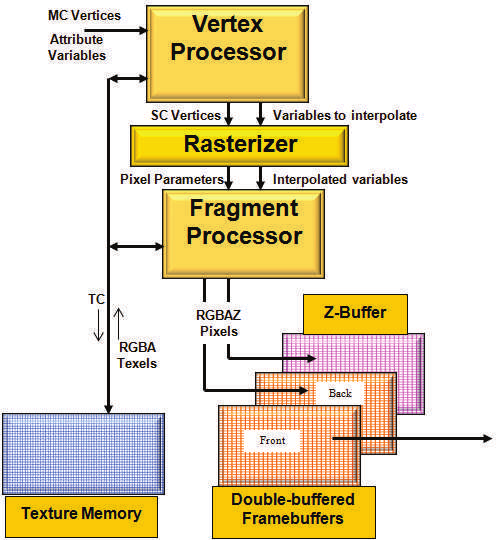
\includegraphics[height=8cm]{figures/pipeline.png}
		\caption{Pipeline de OpenGL}
		\label{fig2.2a}
	\end{subfigure}
	\begin{subfigure}[b]{.5\textwidth}
		\centering
		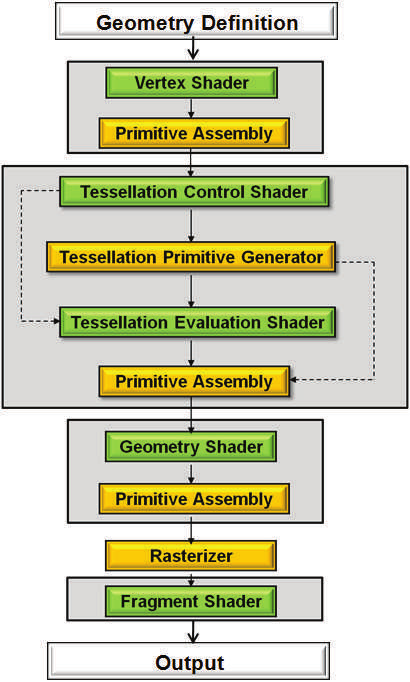
\includegraphics[height=8cm]{figures/pipelineExtendido.png}
		\caption{Pipeline detallado}
		\label{fig2.2b}
	\end{subfigure}
	\caption{Pipeline de gráficos de OpenGL}
	\label{fig2.2}
\end{figure}

El renderizado de una imagen comienza con una llamada, desde la aplicación
principal, a una función de dibujado de OpenGL. Con esta llamada, OpenGL coge
datos sobre vértices contenidos en diferentes objetos y renderiza con estos
datos una o más \textit{primitivas}~\cite{Primitivas}. 

Las primitivas geométricas son las interpretaciones que OpenGL puede
hacer sobre lo que representa un flujo de vértices. Por ejemplo, tres vértices
pueden significar tres puntos independientes, dos líneas, un triángulo, etc.
OpenGL contiene los siguientes tipos principales de primitivas:

\subsection{Primitivas de Puntos}
\label{ref:points}

OpenGL contiene una única primitiva de puntos: \verb|GL_POINTS|. Cuando se llama
a una función de dibujado con esta primitiva, OpenGL interpreta el flujo de
vértices como puntos independientes.

\subsection{Primitivas de Línea}
\label{ref:lines}

En cuanto a las primitivas de línea, hay tres tipos, basándose en distintas
interpretaciones del flujo de vértices.

\begin{itemize}
		\item \verb|GL_LINES|: Los dos primeros vértices se consideran una línea,
				los dos siguientes otra línea, etc.
		\item \verb|GL_LINE_STRIP|: Los vértices adyacentes se consideran una
			línea. Es decir el primero y el segundo forman una línea, el segundo
			y el tercero forman otra línea, etc.
		\item \verb|GL_LINE_LOOP|: Como \verb|GL_LINE_STRIP|, pero el primer y
				último vértices se consideran también una línea.
\end{itemize}

\subsection{Primitivas de Triángulo}
\label{ref:triangles}

Un triángulo es una primitiva formada por tres vértices. También existen tres
primitivas de triángulo:

\begin{itemize}
		\item \verb|GL_TRIANGLES|: los tres primeros vértices forman un
				triángulo, los tres siguientes otro, etc.
		\item \verb|GL_TRIANGLE_STRIP|: cada grupo de tres vértices adyacentes
				forman un triángulo. El (0, 1, 2), el (1, 2, 3), etc.
		\item \verb|GL_TRIANGLE_FAN|: El primer vértice queda fijo, y cada grupo
				de dos vértices adyacentes a partir de él forma un triángulo con
				el primero. Por ejemplo el (0, 1, 2), (0, 2, 3), etc.
\end{itemize}

En la Figura~\ref{fig:primitives} se pueden ver las diferentes interpretaciones
en forma de primitiva que puede realizar OpenGL para renderizar un flujo de
vértices. 

\begin{figure}[h]
	\centering	
	
\includegraphics[width=\textwidth]{figures/primitives.png}
	\caption{Primitivas de OpenGL}
	\label{fig:primitives}
\end{figure}

Una vez se ha hecho la llamada a la función de dibujado, comienza el proceso de
renderizado, recorriéndose las diferentes etapas que forman el pipeline de
renderizado. 

\subsection{Procesamiento de Vértices}
\label{ref:procesamiento}

La primera etapa del pipeline programable ---Vertex Processor,
Figura~\ref{fig2.2a}---, está formada a su vez por los shaders programables de
vértice, teselación y geométrico, que sustituyen a las etapas de transformación
e iluminación del pipeline no programable, así como la etapa fija realizada por
OpenGL conocida como Ensamblado de Primitivas. Obtiene como entrada el flujo de
vértices, normales, definiciones de primitivas geométricas, colores, parámetros
de iluminación, materiales y coordenadas para las texturas. Esta etapa opera
sobre estos datos y los organiza en las primitivas geométricas asociadas en
preparación para la etapa de post-procesado de vértices, en la que se realizan,
entre otras cosas, su recorte y rasterización.  Así, la salida es un conjunto de
vértices como píxeles, con su color, profundidad y coordenadas de textura.

\subsection{Clipping}
\label{ref:clipping}

Posteriormente se realiza el recorte o \textit{clipping}, que ocurre cuando,
ocasionalmente, algunos vértices quedan fuera de lo que se denomina
\textit{viewport}---la región de la ventana donde se permite dibujar---
modificando las primitivas geométricas para que nada quede fuera de ese espacio.
(Ver Figura~\ref{fig2.3a}).

\begin{figure}[h]
	\begin{subfigure}[b]{0.5\textwidth}
		\centering 
		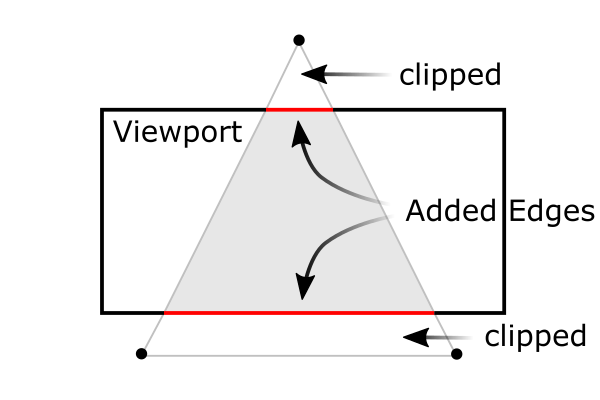
\includegraphics{figures/clipping.png}
		\caption{Clipping en OpenGL}
		\label{fig2.3a}
	\end{subfigure}
	\begin{subfigure}[b]{0.5\textwidth}
		\centering 
		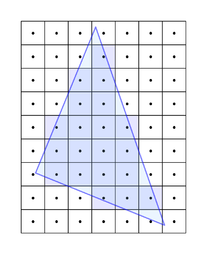
\includegraphics{figures/rasterization.png}
		\caption{Rasterización en OpenGL}
		\label{fig2.3b}
	\end{subfigure}
	\caption{Clipping y rasterización en OpenGL}
	\label{fig2.3}
\end{figure}

\subsection{Rasterización}
\label{ref:rasterizacion}

La siguiente etapa es la rasterización (ver Figura~\ref{fig2.3b}). Este paso
implementa la transición de vértice a fragmento. Inmediatamente después del
clipping, las primitivas geométricas actualizadas se mandan al rasterizador para
la generación de fragmentos. Podemos considerar un fragmento como un ``candidato
a pixel'', en el sentido de que un pixel reside en el \textit{framebuffer}--- un
espacio de memoria manejado por el hardware gráfico que manda al dispositivo de
salida digital--- mientras que un fragmento puede ser rechazado y nunca
actualizar su localización de pixel asociada. 

\subsection{Procesamiento de Fragmentos}
\label{ref:procesamientofrags}

En la última etapa, el procesado de fragmentos se realiza a su vez en dos pasos,
uno de ellos programable con el shader de fragmentos y otras operaciones sobre
fragmentos realizadas automáticamente por OpenGL.  Durante este último
procesamiento, la visibilidad de cada fragmento es determinada utilizando
diferentes tests (profundidad, color, plantilla, ruido\ldots). 

Cuando un fragmento pasa por todas estas etapas y todos los test activos, puede
ser escrito directamente en el buffer de fragmentos, actualizando su color y
valor de profundidad de su pixel o, si el \textit{blending} está activado,
mezclando su color con el del pixel actual para generar un nuevo color que se
escribe en el buffer de fragmentos.

\section{Diferencias con Direct3D}
\label{makereference2.4}

Direct3D es parte del conjunto de la API multimedia DirectX, propiedad de
Microsoft~\cite{Microsoft}. Es la principal competidora de OpenGL, ofreciendo
ambas un conjunto similar de funcionalidades. Aun así, se pueden observar varias
diferencias en términos de disponibilidad, portabilidad, facilidad de uso,
rendimiento, estructura y usuarios finales. En la tabla~\ref{tabla2.1}, se
muestran algunas de ellas resumidas.

\begin{table}[h]
	\centering
	\begin{tabular}{ | m{4cm} | m{5cm} | m{5cm} | }
		\hline
		& OpenGL & Direct3D \\
		\hline
		Soporte de escritorio & Multiplataforma & Microsoft Windows Xbox
		\\
		\hline
		Soporte sistemas empotrados & Multiplataforma (OpenGL ES) & Windows
		Embedded Windows CE \\
		\hline
		Licencia & Libre (con características patentadas) & Privativa
		\\
		\hline
		Usuario final & Profesionales & Juegos \\ 
		\hline
	\end{tabular}
	\caption{Diferencias entre OpenGL y Direct3D}
	\label{tabla2.1}
\end{table}

En cuanto a la portabilidad, DirectX solo está disponible para la familia de
sistemas operativos Microsoft Windows, mientras que OpenGL tiene
implementaciones en muchas plataformas, incluyendo Microsoft Windows y sistemas
Unix.

En términos de facilidad de uso hoy en día ambas APIs se encuentran bastante
parejas, habiendo evolucionado desde las primeras versiones, en las que los
desarrolladores instaban a Microsoft a unirse a la iniciativa OpenGL, debido a
que suponía menos esfuerzo trabajar con esta última.

\begin{figure}
	\centering
	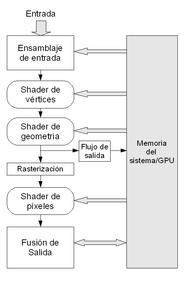
\includegraphics[height=10cm]{figures/directxpipeline.png}
	\caption{Pipeline de gráficos de Direct3D}
	\label{fig:differences}
\end{figure}

El diseño de ambas es también similar. Tras muchos años de evolución, el
pipeline gráfico es bastante parecido, como puede apreciarse en la
Figura~\ref{fig:differences}.

En conclusión, hoy en día ambas se consideran bastante similares en cuanto a
rendimiento y capacidades, siendo el soporte a otros sistemas y el carácter de
las licencias las únicas grandes diferencias que hacen decantarse a los
desarrolladores por una u otra.
